\chapter{Message Passing 
(Belief Propagation)}\label{ch-mp}

Message Passing (aka Belief Propagation)
was first proposed in 1982
Ref.\cite{pearl1982reverend} by Judea Pearl
to simplify
the exact evaluation of probability marginals
of bnets (exact inference).
It gives exact results for trees and
polytrees (i.e. bnets with
a single connected component and
 no acyclic
loops). For bnets with loops,
it gives approximate results 
(loopy belief propagation),
and it has been generalized to
the junction tree algorithm 
(see Chapter \ref{ch-junc-tree})
which can do exact inference
for general bnets with loops.
The basic idea behind
the junction tree algorithm
is to eliminate 
loops by clustering
them into single nodes.

For more information
about Belief Propagation,
see Ref.\cite{wiki-mp}.


\section*{Pearl MP for arbitrary bnets}



Consider Fig.\ref{fig-pi-lam},
which illustrates
a bnet node $\rvx$ receiving and sending
messages to its neighbors.

Note that in Fig.\ref{fig-pi-lam}, 
a function is labeled
$\lam$ (a likelihood
function)  if the
message direction,
 and the  graph arrow,
 point in opposite directions
(i.e, message ``swimming upstream"),
whereas a 
function is labeled $\pi$
(a probability function)  if 
they point in the same direction
(i.e, message ``swimming downstream").
In the symbols $\rcond$
and $\lcond$, the arrow
indicates  the direction of the message,
whereas the vertical line indicates
the direction of the graph arrow.
For  example, in 
$\lam_{\rvb\rcond\rvx}(x)$
the message goes from
$\rvb$ to $\rvx$ and the 
graph arrow
points in the opposite direction.
In 
$\pi_{\rvb\lcond\rvx}(x)$
the message goes from
$\rvx$ to $\rvb$ and the 
graph arrow
points in the same direction.
The argument of the $\pi$
and $\lam$
functions is always the same 
as the letter in the subscript 
that is closest to argument; i.e., the
letter in the subscript that is
to the right of the vertical bar.

Note that in Fig.\ref{fig-pi-lam},
we indicate
messages that travel 
``downstream" 
(resp., ``upstream"), by
arrows with dashed (resp., dotted)
 lines as shafts.
Mnemonic: think of the shaft as a
 velocity vector field
for the message. 
You travel faster when
you swim downstream as opposed
to upstream.

$pa(\rvx)=$ parents of node $\rvx$

$ch(\rvx)=$ children of node $\rvx$

$nb(\rvx)=pa(\rvx)\cup ch(\rvx)=$ 
neighbors of node $\rvx$



\begin{figure}[h!]
\centering
\includegraphics[width=6in]{mpass/pi-lam.png}
\caption{Node $\rvx$ receiving
and sending messages to
 its neighbors. (neighbors=
parents and children).
} 
\label{fig-pi-lam}
\end{figure}




\hrule\noindent
$\rvx$'s incoming messages (one
comes from
each parent and child of $\rvx$)

\begin{itemize}
\item 
$[\lam_{\rvb\rcond\rvx}(\cdot)]_
{\rvb\in ch(\rvx)}$
\item
$[\pi_{\rvx\lcond\rva}(\cdot)]_
{\rva\in  pa(\rvx)}$
\end{itemize}

\beqa
IN_\rvx&=&
([\lam_{\rvb\rcond\rvx}(\cdot)]_
{\rvb\in ch(\rvx)},
[\pi_{\rvx\lcond\rva}(\cdot)]_
{\rva\in  pa(\rvx)})
\\
&=&
[IN_{\rvx,\rvn}]_{\rvn\in nb(\rvx)}
\eeqa

\hrule\noindent
$\rvx$'s outgoing messages
 (one goes to each parent 
and child of $\rvx$)

\begin{itemize}
\item
$[\pi_{\rvb\lcond\rvx}(\cdot)]_
{\rvb\in ch(\rvx)}$
\item 
$[\lam_{\rvx\rcond\rva}(\cdot)]_
{\rva\in  pa(\rvx)}$
\end{itemize}

\beqa
OUT_\rvx&=&
([\pi_{\rvb\lcond\rvx}(\cdot)]_
{\rvb\in ch(\rvx)},
[\lam_{\rvx\rcond\rva}(\cdot)]_
{\rva\in  pa(\rvx)})
\\
&=&
[OUT_{\rvx,\rvn}]_{\rvn\in nb(\rvx)}
\eeqa
\hrule\noindent
$\rvx$'s memory

\beq
\calm_\rvx =
(IN_\rvx,OUT_\rvx)
\eeq

\hrule

For times $t=0, 1, \dots, T-1$,
 we calculate $\calm^{(t)}_\rvx$ in
two steps: first we calculate $IN^{(t)}_\rvx$,
 then
we calculate $OUT^{(t)}_\rvx$:

\begin{figure}[h!]
\centering
\includegraphics[width=3.5in]
{mpass/mpass-messages.png}
\caption{The yellow
node is a gossip monger.
It receives messages from
all the green nodes,
and then it relays a joint
message to the red node.
Union of green nodes and the red node = full
 neighborhood of yellow node.
There are two possible 
cases: the
red node is either a parent 
or a child of the yellow 
one. As usual, we use arrows with
dashed (resp., dotted) shafts for
downstream (resp., upstream) messages.  } 
\label{fig-messages-gen}
\end{figure}



\begin{enumerate}
\item {\bf Calculating 
$IN^{(t)}_\rvx$
from signals received from
 $\rvn\in R\subset nb(\rvx)$:}

For all $\rvn\in nb(\rvx)$,
\beq
IN^{(t)}_{\rvx, \rvn}=\left\{
\begin{array}{l}
IN^{(t-1)}_{\rvx, \rvn}
\text{ if $\rvn\notin R$}
\\
OUT^{(t-1)}_{\rvn,\rvx}
 \text{ if $\rvn\in R$}
\end{array}
\right.
\eeq

No instantaneous replies (message backflow):
If $\rvx$ receives signals
from $R\subset nb(\rvx)$
and sends them to
$S\subset nb(\rvx)$,
then $S$ and $R$
are disjoint and 
 $R\cup S=nb(\rvx)$.

\item {\bf Calculating $OUT_\rvx^{(t)}$
from already calculated $IN_\rvx^{(t)}$:}

Let $\rva^{na}=
(\rva_i)_{i=0, 1, \ldots, na-1}$
denote the parents of $\rvx$
and
$\rvb^{nb}=
(\rvb_i)_{i=0, 1, \ldots, nb-1}$
its children.

Define

\beqa
\pi_{\rvx\lcond}(x)&=&
\sum_{a^{na}} P(x|a^{na})
\prod_i
\pi_{\rvx\lcond\rva_i}
(a_i)\\
&=&E_{\rva^{na}}[P(x|a^{na})]
\eeqa
and

\beq
\lam_{\rcond\rvx}(x)=
\prod_i
\lam_{\rvb_i\rcond \rvx}(x)
\;.
\eeq

From 
the $m_{\rva \larrow\rvx}$
panel of Fig.\ref{fig-messages-gen}, 
 we get\footnote{As usual in this book,
$\caln(!x)$ means
a constant that is independent of $x$.}

\beqa
\underbrace{\lam_{\rvx\rcond\rva_i}
(a_i)}_{OUT}&=&
\caln(!a_i)
\sum_x\left[
\underbrace{\lam_{\rcond\rvx}(x)}_{IN}
\sum_{(a_k)_{k\neq i}}\left(
P(x|a^{na})\prod_{k\neq i}
\underbrace{\pi_
{\rvx\lcond\rva_k}
(a_k)}_{IN}
\right)\right]
\\&=&
\caln(!a_i)
\sum_x\left[
\lam_{\rcond\rvx}(x)
E_{(\rva_k)_{k\neq i}}[P(x|a^{na})]\right]
\\&=&
\caln(!a_i)
E_{(\rva_k)_{k\neq i}}E_{\rvx|a^{na}}
\lam_{\rcond\rvx}(x)
\eeqa

From the $m_{\rvb \larrow\rvx}$
panel of
Fig.\ref{fig-messages-gen}, 
we get


\beq
\underbrace{\pi_{\rvb_i\lcond\rvx}
(x)}_{OUT}=
\caln(!x)
\underbrace{\pi_{\rvx\lcond}(x)}_{IN}
\prod_{k\neq i}
\underbrace{\lam_{\rvb_k\rcond \rvx}(x)}_{IN}
\eeq
\end{enumerate}


\hrule\noindent
{\bf Claim:} Define

\beq
BEL^{(t)}(x)=\caln(!x)
\lam^{(t)}_{\rcond\rvx}(x)
\pi^{(t)}_{\rvx\lcond}(x)
\;.\eeq
Then

\beq
\lim_{t\rarrow \infty}BEL^{(t)}(x)=P(x)
\;.
\eeq
This  says that
the belief in $\rvx=x$
converges to $P(x)$ and it
equals the product 
of messages received from all
parents and children of $\rvx=x$.


\hrule
\section*{Example of Pearl MP}

\begin{figure}[h!]
\centering
$$\xymatrix{
\rvA\ar[d]\ar[dr]
\\
\rvA_{0}\ar[d]\ar[dr]
&\rvA_{1}\ar[dr]\ar[drr]
\\
\rvA_{00}
&\rvA_{01}
&\rvA_{10}
&\rvA_{11}
}$$
\caption{bnet for a full binary 
tree with 3 levels. $\rvA$ is
the apex root node.}
\label{fig-full3-tree}
\end{figure}

\begin{figure}[h!]
\centering
$$\xymatrix{
\rvA\ar[d]\ar@/_2pc/[dd]
&\ucalm_\rvA^{(0)}\ar[rd]\ar[rdd]
\ar[r]
&\ucalm_\rvA^{(1)}
\ar[r]
&\ucalm_{\rvA}^{(2)}
\\
\rvA_{0}\ar@/_2pc/[dd]\ar@/_2pc/[ddd]
&\ucalm_{\rvA_{0}}^{(0)}
\ar[r]
&\ucalm_{\rvA_{0}}^{(1)}
\ar[r]\ar[rddd]\ar[rdd]
&\ucalm_{\rvA_{0}}^{(2)}
\\
\rvA_{1}\ar@/_2pc/[ddd]\ar@/_2pc/[dddd]
&\ucalm_{\rvA_{1}}^{(0)}
\ar[r]
&\ucalm_{\rvA_{1}}^{(1)}
\ar[rddd]\ar[rdddd]
\ar[r]
&\ucalm_{\rvA_{1}}^{(2)}
\\
\rvA_{00}
&\ucalm_{\rvA_{00}}^{(0)}
\ar[r]
&\ucalm_{\rvA_{00}}^{(1)}
&\ucalm_{\rvA_{00}}^{(2)}
\\
\rvA_{01}
&\ucalm_{\rvA_{01}}^{(0)}
\ar[r]
&\ucalm_{\rvA_{01}}^{(1)}
\ar[r]
&\ucalm_{\rvA_{01}}^{(2)}
\\
\rvA_{10}
&\ucalm_{\rvA_{10}}^{(0)}
\ar[r]
&\ucalm_{\rvA_{10}}^{(1)}
\ar[r]
&\ucalm_{\rvA_{10}}^{(2)}
\\
\rvA_{11}
&\ucalm_{\rvA_{11}}^{(0)}
\ar[r]
&\ucalm_{\rvA_{11}}^{(1)}
\ar[r]
&\ucalm_{\rvA_{11}}^{(2)}
}$$
\caption{messages-bnet
for the source-bnet Fig.\ref{fig-full3-tree}.}
\label{fig-mp-bnet-for-tree}
\end{figure}
Fig.\ref{fig-mp-bnet-for-tree} 
is the {\bf messages-bnet}
 for the 
{\bf source bnet} Fig.\ref{fig-full3-tree}.
The node TPMs,
printed in blue,
for the bnet
Fig.\ref{fig-mp-bnet-for-tree},
are as follows.


The following equation
applies with  $t=1$,
and $\rvx\in\{\rvA_0, \rvA_1\}$.
It also applies with
 $t=2$ and $\rvx\in\{
 \rvA_{00},\rvA_{01},
\rvA_{10},\rvA_{11}\}$.

\beqa\color{blue}
P(\calm_{\rvx}^{(t)}\cond 
[\calm_{\rva}^{(t-1)}]_
{\rva\in pa(\rvx)\cup \rvx})&=&\color{blue}
\delta(
\calm_{\rvx}^{(t)},
\calm_{\rvx}^{(t)}
( 
[\calm_{\rva}^{(t-1)}]_
{\rva\in pa(\rvx)\cup   \rvx})
)
\eeqa

Whenever the only arrow
entering $\calm_{\rvx}^{(t)}$
is from $\calm_{\rvx}^{(t-1)}$,
there is no change in $\calm_{\rvx}^{(t)}$:

\beq\color{blue}
P(\calm_{\rvx}^{(t)}\cond
\calm_{\rvx}^{(t-1)})=
\delta(
\calm_{\rvx}^{(t)},
\calm_{\rvx}^{(t-1)})
\;.
\eeq

As for the root nodes
of the messages-bnet  at time $t=0$,
they should encode the prior
prob  distributions
of the source bnet Fig.\ref{fig-full3-tree}.
In this example, the only root node 
of the source bnet is $\rvA$. Thus, let

\beq
IN^{(0)}_\rvA=0,\;\;
OUT^{(0)}_\rvA= P_\rvA(\cdot),\;\;
\calm^{(0)}_\rvA=(IN^{(0)}_\rvA,OUT^{(0)}_\rvA)
\eeq

\beq\color{blue}
P(\calm^{(0)}_\rvA)=
\delta(\calm^{(0)}_\rvA,
\calm^{(0)}_\rvA(\ldots))
\;.
\eeq


\begin{figure}[h!]
\centering
$$
\begin{array}{cc}
\xymatrix{
\rvA\ar[d]\ar[dr]
\ar@[red]@{-->}@<2ex>[d]
\ar@[red]@{-->}@<2ex>[dr]
\\
\rvA_{0}\ar[d]\ar[dr]
&\rvA_{1}\ar[dr]\ar[drr]
\\
\rvA_{00}
&\rvA_{01}
&\rvA_{10}
&\rvA_{11}
}
&
\xymatrix{
\rvA\ar[d]\ar[dr]
\\
\rvA_{0}\ar[d]\ar[dr]
\ar@[red]@{-->}@<2ex>[d]
\ar@[red]@{-->}@<2ex>[dr]
&\rvA_{1}\ar[dr]\ar[drr]
\ar@[red]@{-->}@<2ex>[dr]
\ar@[red]@{-->}@<2ex>[drr]
\\
\rvA_{00}
&\rvA_{01}
&\rvA_{10}
&\rvA_{11}
}
\\
\text{t= 0-1}&\text{t= 1-2}
\end{array}
$$
\caption{
The messages passed in 
Fig.\ref{fig-mp-bnet-for-tree}
are indicated by red arrows
on the source bnet 
Fig.\ref{fig-full3-tree}.
As usual, we use arrows with
dashed (resp., dotted) shafts for
downstream (resp., upstream) messages. 
In this diagram, there are only
dashed arrows.
}
\label{fig-full3-tree-messages}
\end{figure}

If the state of a node
is known a priori (i.e., 
there is a prior  ``evidence"
for that node),
then,
in the MP procedure,  replace that
node's TPM by
a Kronecker delta function.
$BEL^{(t)}(x)$ should
now  converge to $P(x|\text{ a priori
evidence for
 all nodes})$.

In Fig.\ref{fig-full3-tree-messages},
the messages passed in the messages-bnet
are indicated by red arrows
on the source bnet.



\newpage
\section*{Bipartite bnets}

By a {\bf bipartite bnet}
we will mean a bnet
all of whose nodes 
are root nodes (parentless)
or leaf nodes (childless).
Pearl MP  
simplifies when dealing with 
bipartite bnets. In this section,
we will explain how
it simplifies. But
before doing so,
let us explain how the 
following two types of
diagrams
can be replaced by
equivalent bipartite bnets:

\begin{itemize}
\item Factor Graphs
\item Tree bnets
\end{itemize}
\hrule

Consider a product $g=\prod_\alp f_\alp$
of scalar functions
 $f_\alp:\RR^{nx(\alp)}\rarrow \RR$
for $\alp=0, 1, \ldots nf-1$. For instance, 
consider $g:\RR^3\rarrow \RR$
defined by:

\beq
g(x_0,x_1,x_2) = f_0(x_0)
f_1(x_0,x_1)f_2(x_0,x_1)f_3(x_1,x_2)
\label{eq-g-fun}
\;.
\eeq
The {\bf factor graph}
for this function $g$
 is given by Fig.\ref{fig-fac-graph}.


\begin{figure}[h!]
\centering
$$\xymatrix{
*++[o][F]{x_0}\ar@{-}[d]\ar@{-}[dr]\ar@{-}[drr]
&*++[o][F]{x_1}\ar@{-}[d]\ar@{-}[dr]\ar@{-}[drr]
&*++[o][F]{x_2}\ar@{-}[dr]
\\
*+[F]{f_0}
&*+[F]{f_1}
&*+[F]{f_2}
&*+[F]{f_3}
}$$
\caption{Factor graph for function
$g$ defined by Eq.(\ref{eq-g-fun}).}
\label{fig-fac-graph}
\end{figure}

\begin{figure}[h!]
\centering
$$\xymatrix{
\rvx_0\ar[d]\ar[dr]\ar[drr]
&\rvx_1\ar[d]\ar[dr]\ar[drr]
&\rvx_2\ar[dr]
\\
\rvf_0&\rvf_1&\rvf_2&\rvf_3
}$$
\caption{Bipartite bnet
corresponding to factor 
graph Fig.\ref{fig-fac-graph}.}
\label{fig-bip-bnet}
\end{figure}

One
can map
any factor graph (the ``source")
to a special bipartite bnet (the ``image"),
as follows.
Replace each $x_i$ by $\rvx_i\in\RR$
for $i=0,1, \ldots, nx-1$
 and each
 $f_\alpha$ by $\rvf_\alpha\in \RR$
for $\alpha=0, 1, \ldots, nf-1$.
Then replace
the connections (edges)
of the factor graph
by arrows from $\rvx_i$ to
$\rvf_\alpha$. For example,
Fig.\ref{fig-bip-bnet}
is the image of the factor 
graph Fig.\ref{fig-fac-graph}.


Let $\rvx^{nx}=
(\rvx_0, \rvx_1, \ldots, \rvx_{nx-1})$,
$\rvf^{nf}=
(\rvf_0, \rvf_1, \ldots, \rvf_{nf-1})$,
and $f_\alp=f_\alp(x_{nb(\rvf_\alp)})$.
Here we are using $nb(\rvf_\alp)$
to denote  the neighborhood
of node $\rvf_\alp$
in the image bipartite bnet,
and we are using $x_S$ to denote
$(x_i)_{i\in S}$.
Then we define the node TPMs, printed
in blue, for the
image bipartite bnet, to be




\beq\color{blue}
P(f_\alpha|x_{nx(\rvf_\alpha)})= 
\caln(!x_{nb(\rvf_\alpha)})
f_\alpha(x_{nb(\rvf_\alpha)})
\;
\eeq
for $\alp=0, 1, \ldots , nf-1$
and

\beq\color{blue}
P_{\rvx_i}(x_i')=\delta(x_i', x_i)
\eeq
for $i=0, 1, \ldots, nx-1$.

Note that

\beq
P(f^{nf}|x^{nx})=
\caln(!x^{nx})
\prod_\alpha 
f_\alpha(x_{nb(\rvf_\alpha)})
\;.
\eeq

\hrule
A {\bf tree bnet}
is a bnet for which all 
nodes have exactly
one parent except
for the apex root 
node which has none.
A tree bnet 
is very much like
the filing system 
in a computer.

One can map a tree
 bnet (the ``source")
into
an equivalent
bipartite bnet (the ``image") as follows.
Replace
each arrow

\beq
\xymatrix{
\rvx\ar[rr]&&\rvy
}
\eeq
of the tree bnet by


\beq
\xymatrix{
\rvx\ar[r]
&
\ul{P_{\rvy|\rvx}}
&
\rvy\ar[l]
}\;.
\eeq
For example,
the tree bnet Fig.\ref{fig-part3-tree}
has the image 
bipartite bnet given by
Fig.\ref{fig-part3-tree-junc-tree}.
The
bnet Fig.\ref{fig-part3-tree-bip-bnet}
is just
a different
way of drawing the bnet
Fig.\ref{fig-part3-tree-junc-tree}.

\begin{figure}[h!]
$$\xymatrix{
\rvA\ar[d]\ar[rrd]
\\
\rvA_0\ar[d]\ar[rd]&&\rvA_1
\\
\rvA_{00}&\rvA_{01}
}
$$
\caption{Example of a tree bnet.}
\label{fig-part3-tree}
\end{figure}


\begin{figure}[h!]
$$\xymatrix{
\rvA\ar[d]\ar[rrd]
\\
\ul{P_{\rvA_0|\rvA}}&&\ul{P_{\rvA_1|\rvA}}
\\
\rvA_0\ar[u]\ar[d]\ar[rd]&&\rvA_1\ar[u]
\\
\ul{P_{\rvA_{00}|\rvA_0}}&\ul{P_{\rvA_{01}|\rvA_0}}
\\
\rvA_{00}\ar[u]&\rvA_{01}\ar[u]
}
$$
\caption{Bipartite bnet
corresponding
to tree bnet Fig.\ref{fig-part3-tree}.}
\label{fig-part3-tree-junc-tree}
\end{figure}

\begin{figure}[h!]
\centering
$$\xymatrix{
\rvA\ar[dr]\ar[drr]
&\rvA_{0}\ar[d]\ar[drr]\ar[drrr]
&\rvA_{1}\ar[d]
&\rvA_{00}\ar[d]
&\rvA_{01}\ar[d]
\\
&\ul{P_{\rvA_{0}|\rvA}}
&\ul{P_{\rvA_{1}|\rvA}}
&\ul{P_{\rvA_{00}|\rvA_0}}
&\ul{P_{\rvA_{01}|\rvA_0}}
}$$
\caption{
Different
way of drawing 
the bnet Fig.\ref{fig-part3-tree-junc-tree}.}
\label{fig-part3-tree-bip-bnet}
\end{figure}

The node  TPMs, printed in blue,
for the image bipartite bnet 
Fig.\ref{fig-part3-tree-junc-tree},
are as follows. We express the
TPMs of the image bnet
in terms of the 
TPMs of the source bnet 
Fig.\ref{fig-part3-tree}.

\beq\color{blue}
P(P_{\rvy|\rvx}| x, y)=P_{\rvy|\rvx}(y|x)
\eeq
for all the
\ul{leaf} 
nodes $P_{\rvy|\rvx}$ of the
image bipartite bnet.
Also

\beq\color{blue}
P_\rvy(y')= \delta(y', y)
\;
\eeq
for all the \ul{root} nodes $\rvy$ of the
image bipartite bnet
except when 
$\rvy$ corresponds to
the root node $\rvA$
of the source tree bnet.
In that exceptional case,

\beq\color{blue}
P_\rvy(y')= P_\rvA(y')
\;.
\eeq


\hrule


\section*{MP for
bipartite bnets}
For
a bipartite 
bnet as defined before,
with
root nodes $\rvx_i$
and leaf nodes $\rvf_\alp$,
let


\beq
nb(i)=\{\alp: \rvf_\alpha\in
nb(\rvx_i)\}
\;,
\eeq

\beq
nb(\alpha)=\{i: \rvx_i\in
nb( \rvf_\alpha)\}
\;,
\eeq

\beq
m_{\alp\larrow i}
(x_i)
=
\pi_{\rvf_\alpha \lcond\rvx_i }
(x_i)
\;,
\eeq

\beq
m_{i\larrow \alp}
(x_i)
=
\lam_{\rvf_\alp\rcond \rvx_i}
(x_i)
\;,
\eeq


\begin{figure}[h!]
\centering
\includegraphics[width=3.5in]
{mpass/mpass-messages-bip.png}
\caption{This figure is equivalent to
Fig.\ref{fig-messages-gen}
for the special case of a 
bipartite bnet. Union of green nodes and the red node = full
 neighborhood of yellow node.
There are two possible 
cases:  the
red node is either a parent
or a child  of the yellow 
node.}  
\label{fig-messages-bip}
\end{figure}

Next we will
show how
to find $m_{\alp\larrow i}^{(t)}$
and $m_{i\larrow \alp}^{(t)}$
from other messages at times
 $t$ and  $t-1$.

\begin{enumerate}

\item {\bf 
We find $m_{\alp\larrow i}^{(t)}$
 as follows.}

See 
the 
$m_{\rvf_2\larrow\rvx_1 }$ panel of
Fig.\ref{fig-messages-bip}.

For $i=0, 1, \ldots , nx-1$, if
 $\alp\in nb(i)$, then

\beq
m^{(t)}_{\alp\larrow i }(x_i)
=
\prod_{
\beta\in nb(i)-\alpha}
m^{(t-1)}_{i\larrow \beta}(x_i)
\;,
\label{eq-mp-iter1}
\eeq
whereas if  $\alp\notin nb(i)$ 

\beq
m^{(t)}_{\alp\larrow i}=
m^{(t-1)}_{\alp\larrow i}
\;.
\eeq

\item {\bf
We find $m_{i\larrow \alp}^{(t)}$ as follows.}

See the
$m_{\rvx_2\larrow\rvf_1 }$ panel
of Fig.\ref{fig-messages-bip}.

For $\alp=0, 1, \ldots, nf-1$, if
 $i\in nb(\alp)$, then


\beqa
m^{(t)}_{i\larrow \alp}(x_i)
&=&
\sum_{(x_k)_{k\in nb(\alpha)-i}}
f_\alpha(x_{nb(\alpha)})
\prod_{k\in nb(\alpha)-i}
m^{(t-1)}_{\alp\larrow k }
(x_k)
\\
&=&
E^{(t-1)}_{(x_k)_{k\in nb(\alpha)-i}}[
f_\alpha(x_{nb(\alpha)})]
\;,
\label{eq-mp-iter2}
\eeqa
whereas if $i\notin nb(\alp)$

\beq
m^{(t)}_{i\larrow \alp}(x_i)
=
m^{(t-1)}_{i\larrow \alp}(x_i)
\;.
\eeq

\end{enumerate}

In the above
equations for
$m_{\alp\larrow i}^{ (t)}$
and $m_{i\larrow \alp}^{ (t)}$, if the
range set of a product is empty, then
 define the product as 1; i.e., 
$\prod_{k\in \emptyset}F(k)=1$.



\hrule\noindent
{\bf Claim:}

\beq
P(x_i)=
\lim_{t\rarrow 
\infty}\caln(!x_i)\prod_{\alp\in nb(i)}
m^{(t)}_{i\larrow \alp}(x_i)
\;
\label{eq-m-prod}
\eeq
and

\beq
P(x_{nb(\alp)})=\lim_{t\rarrow \infty}
\caln(!x_{nb(\alp)})
f_\alp(x_{nb(\alp)})
\prod_{i\in nb(\alp)}
m^{(t)}_{\alp\larrow i}(x_i)
\;.
\label{eq-f-m-prod}
\eeq
\hrule

Eq.(\ref{eq-m-prod})
and the recursive  message
passing equations
that yield
the messages
on the right hand side of
Eq.(\ref{eq-m-prod}), together
yield what
is often
referred to as 
a {\bf  sum-product decomposition}.
I don't like that name 
because it is unnecessarily
confusing and it fails to convey the
recursive nature of the decomposition.
I prefer to call it a {\bf
recursive sum of products 
(RSOP) decomposition},
and will call it so henceforth
in this chapter.

Expressing the marginals of a bnet
as RSOPs,
which is what MP does,
reduces the complexity 
of the calculation.
(i.e.,
the total number
of additions
and multiplications
that need to be performed)
That makes 
using the MP
algo very advantageous.




Note that given
a function $g:\RR^{nx}\rarrow \RR$,
one can find
$\argmax_{x^{nx}} g(x^{nx})$ (or
argmin)
by replacing all
sums over $x$
components by argmax's (or argmin's)
in the MP algorithm.



\section*{Example of MP for
bipartite bnets}

Consider
the bipartite
bnet \ref{fig-part3-tree}. 
We define its messages-bnet
to be Fig.\ref{fig-part3-tree-mp-bnet}.
For that messages-bnet, 
the node TPMs, printed in blue,
are as follows.
They come directly
from Eqs.(\ref{eq-mp-iter1}
and (\ref{eq-mp-iter2}).

\beq\color{blue}
P(A) = P_\rvA(A)
\eeq

\beq\color{blue}
P(m^{(t)}_{i\larrow \alp}(\cdot)\cond
pa[m^{(t)}_{i\larrow \alp}(\cdot)]
)=
\indi(\;\;\;
m^{(t)}_{i\larrow \alp}(x_i)
=
E^{(t-1)}_{(x_k)_{k\in nb(\alpha)-i}}[
f_\alpha(x_{nb(\alpha)})]
\;\;\;)
\eeq

\beq\color{blue}
P(
m^{(t)}_{\alp\larrow i }(\cdot)
\cond
pa[m^{(t)}_{\alp\larrow i }(\cdot)]
)
=
\indi(\;\;\;
m^{(t)}_{\alp\larrow i }(x_i)
=
\prod_{
\beta\in nb(i)-\alpha}
m^{(t-1)}_{i\larrow \beta}(x_i)
\;\;\;)
\eeq


\begin{figure}[h!]
$$\xymatrix{
\rvA\ar[d]\ar[rrd]
\\
m^{(1)}_{\ul{P_{\rvA_0|\rvA}}\larrow\rvA}\ar[d]
&&
m^{(1)}_{\ul{P_{\rvA_1|\rvA}}\larrow\rvA}\ar[d]
\\
mm^{(2)}_{\rvA_0\larrow \ul{P_{\rvA_0|\rvA}}}
\ar[d]\ar[dr]
&&
m^{(2)}_{\rvA_1\larrow \ul{P_{\rvA_1|\rvA}}}
\\
m^{(3)}_{
\ul{P_{\rvA_{00}|\rvA_0}}\larrow \rvA_0}\ar[d]
&
m^{(3)}_{
\ul{P_{\rvA_{01}|\rvA_0}}\larrow \rvA_0}\ar[d]
\\
m^{(4)}_{\rvA_{00}
\larrow \ul{P_{\rvA_{00}|\rvA_0}}}
&m^{(4)}_{\rvA_{00}
\larrow \ul{P_{\rvA_{01}|\rvA_0}}}
}
$$
\caption{messages-bnet
corresponding
to tree bnet Fig.\ref{fig-part3-tree}.}
\label{fig-part3-tree-mp-bnet}
\end{figure}

Note that 
for the tree bnet 
Fig.\ref{fig-part3-tree}, one has
\beqa
P(A_{00})&=&
\sum_{A, A_0}
P(A_{00}|A_0)P(A_0|A)P(A)
\\
&=&
\sum_{A_0}\left\{
P(A_{00}|A_0)
\sum_A
\left\{
P(A_0|A)P(A)
\right\}
\right\}
\label{eq-sum-p}
\eeqa
The right hand side
of Eq.(\ref{eq-sum-p})
 is expressed as a 
recursive
sum of products (RSOP).
In fact, 
if we consider
the path

\beq
\xymatrix{
\rvA_{00}\ar[r]
&\ul{P_{\rvA_{00}|\rvA_0}}
&\rvA_0\ar[l]\ar[r]
&\ul{P_{\rvA_0|\rvA}}
&\rvA\ar[l]\ar[r]
&\ul{P_\rvA}
}
\eeq
in the bipartite bnet
 Fig.\ref{fig-part3-tree-junc-tree},
we get the same RSOP
from the MP algorithm:

\beq
P(A_{00})=
\caln(!A_{00})
m_{\rvA_{00}\larrow \ul{P_{\rvA_{00}|\rvA_0}}}(A_{00})
\eeq

\beq
m_{\rvA_{00}\larrow \ul{P_{\rvA_{00}|\rvA_0}}}(A_{00})
=
\sum_{A_0}
P(A_{00}|A_0)
m_{\ul{P_{\rvA_{00}|\rvA_0}}\larrow \rvA_0}(A_0)
\eeq

\beq
m_{\ul{P_{\rvA_{00}|\rvA_0}}\larrow \rvA_0}(A_0)
=
m_{\rvA_0\larrow\ul{P_{\rvA_{0}|\rvA}} }(A_0)
\eeq

\beq
m_{\rvA_0\larrow\ul{P_{\rvA_{0}|\rvA}} }(A_0)=
\sum_{A}P(A_0|A)
m_{\ul{P_{\rvA_{0}|\rvA}}\larrow \rvA}(A)
\eeq

\beq
m_{\ul{P_{\rvA_{0}|\rvA}}\larrow \rvA}(A)
=P(A)
\eeq




